\chapter{Systém}

V kapitole \ref{chapter:legal-analysis} sme zanalyzovali právne požiadavky ZoKB a ZoITVS, ktoré nám uložili povinnosť
zaviesť ISMS. V nasledujúcej kapitole \ref{chapter:isms} sme pomocou kompendia IT-Grundschutz\cite{GSK} popísali a
vysvetlili štruktúru ISMS na základnej úrovni. Teraz máme všetko potrebné na to, aby sme navrhli a čiastočne implementovali 
systém pre manažéra KIB, ktorý:

\begin{itemize}
  \item mu poskytne minimálne znalosti v oblasti KIB,
  \item prevedie ho úvodnými krokmi zavádzania ISMS a
  \item pomôže mu zozbierať informácie potrebné na vypracovanie bezpečnostnej dokumentácie\footnote{Konkrétne politiky KIB.}.
\end{itemize}

Pri vypracovaní systému a písaní obsahu sme vychádzali z materiálov a metodík  BSI 200-1\cite{BSI1}, BSI 200-2\cite{BSI2},
BSI 200-3\cite{BSI3}, kompendia IT-Grundschutz\cite{GSK} a IT-Grundschutz-Online-Course\cite{GSK-OC}. Rozhranie systému
je prevedené ako webová aplikácia, beží lokálne na počítači a je sprístupnený cez ľubovoľný prehliadač. Zdrojový kód je
v prílohe a súčasne je zverejnený na GitHub-e \url{https://github.com/AntonKica/spvbp-isvs-portal-backend}.

V tejto kapitole sa ešte budeme venovať technickej špecifikácií, prezentácií výsledného systému, databázovému pohľadu a
ako nakoniec tomu, ako spustiť systém. Teraz by sme sa pozreli na technickú špecifikáciu, nástroje a technológie použité
na vypracovanie systému.

\section{Technická špecifikácia}

Systém je logicky rozdelený na dve vrstvy -- backend a frontend\footnote{Pre slovenských čítateľov sú známejšie v poradí pojmy
serverová časť a klientská časť. My sme sa rozhodli používať anglické výrazy, ktoré nám prišli prirodzenejšie.}. Backend
tvorí logiku systému, spracováva dáta a ukadá ich do databázy. Frontend poskytuje užívateľské rozhranie, užívateľ tu zadáva
vstupné údaje, ktoré sa posielajú backendu na spracovanie. Komunikácia medzi týmito dvoma vrstvami je realizovaná prostredníctvom
protokolu HTTP a RPC\footnote{Z angl. \textit{remote procedure call}, volanie vzdialenej procedúry, vďaka ktorému možno
vykonať kód zo vzdialeného miesta, na inom zariadení.}.

\subsection*{Backend}
Na vývoj backendu sme použili programovací jazyk Java verzie 21 a ekosystém vybudovaný kolo nej. Voľba programovacieho jazyka
bola motivovaná najmä tým, že:
\begin{itemize}
  \item disponujeme znalosťou a skúsenosťou s Javou a jej ekosystémom,
  \item frameworky, knižnice a nástroje Javy boli pre nás nápomocné, pri vývoji podstatných častí systému a
  \item sme nemuseli zbytočne strácať čas nad riešením technických úloh/problémov nesúvisiacimi s našou bakalárskou prácou.
\end{itemize}

Správu knižníc a balíčkov, kompiláciu a spustenie\footnote{Toto do istej miery nie je pravda, keďže na lokálny vývoj sme
použuli integrované vývojové prostredie.} sme vyriešili pomocou nástroja Gradle verzie 8.

So spracovaním RPC sme si pomohli frameworkom Spring Boot verzie 3, ktorý nám tiež pomohol s:
\begin{itemize}
  \item celkovou konfiguráciou backendu,
  \item prehľadným definovaním rozhrania a endpointov\footnote{Koncové body, URL linka v prehliadači.} pre komunikáciu s
    frontendom
  \item serializáciou/deserializáciou vystupných/vstupných dát a
  \item manažmentom tried a repozitárov.
\end{itemize}

Na ukladanie dát systému sme použili SQL databázu PostgreSQL verzie 16. S databázou sme nekomunikovali priamo, ale pomocou
ORM\footnote{Z angl. \textit{object-relation mapping}, objektovo relačné mapovanie, vďaka ktorému sú triedy zmapované
na štruktúry databázy.} frameworku Hibernate verzie 6. Hibernate nám pomohol s opakovaným kódom\footnote{Veľké množstvo
opakovaný kódu je dlhodobá kritika programovacieho jazyka Java.} a pri vývoji systému, hlavne pri zmenách tried\footnote{Nemuseli
sme strácať čas úpravou rozhrania medzi triedami a korešpondujúcimi schémami v databáze.}.

Na testovanie sme využili knižnicu JUnit verzie 5. Avšak, v prebehu vývoja sme zistili, že nie je potrebné písať testy,
ktoré by nás maximálne zdržiavali. Dôvodom bolo to, že pri zmenách kódu sme nepotrebovali kontrolovať funkcionalitu a 
konzistenciu dát\footnote{Pracovali sme sami a chyby sme si ešte vedeli ustrážiť.}.

\subsection*{Frontend}
Na vývoj frontendu sme použili HTML5 a v menšom množstve JavaScript\footnote{Na verziach moc nezáleží, používali sme
funkcionalitu podporovanú väčšinou, ak nie všetkými modernými prehliadačmi.}. Pre dosiahnite krajšieho a estetickejšieho
vzhľadu\footnote{Pre čitateľa zdôraznime, aby od nás nečakal veľmi úhľadné vizuály, že sme informatici, nie grafici.}
sme použili CSS sady nástrojov Bootstrap verzie 5.

Síce sme stránky písali v jazyku HTML, no na ich zobrazenie sme použili šablónovací jazyk a techniku SSR\footnote{Z angl.
\textit{server-side rendering}, spôsob, kde sa celá stránka plne zostaví/vykreslí na strane servera, pričom server zašle
klientovi čistý HTML súbor.}, kde nám opäť pomohol ekosystém Javy. Šablónovací nástroj Thymeleaf verzie 3 nám pomohol so
svojim dialektom HTML prehľadne zobraziť dáta, zoznamy, triedy a definovať si tzv. fragmenty -- vizuálne prvky, ktoré sme mohli
opakovane použiť pri tvorbe jednotlivých stránok.

\section{Prezentácia výsledného systému}
Pomocou nástrojov využitých v backende a frontende sme vytvorili ukážkový systém, s ktorým interaguje používateľ, manažér
KIB. System sa skladá z dvoch hlavných častí, jednej menšej -- úvod (obr. \ref{fig:isms-uvodna-stranka}), a druhej nosnej
-- návod (obr. \ref{fig:isms-setup}).

\begin{figure}[h]
  \centering
  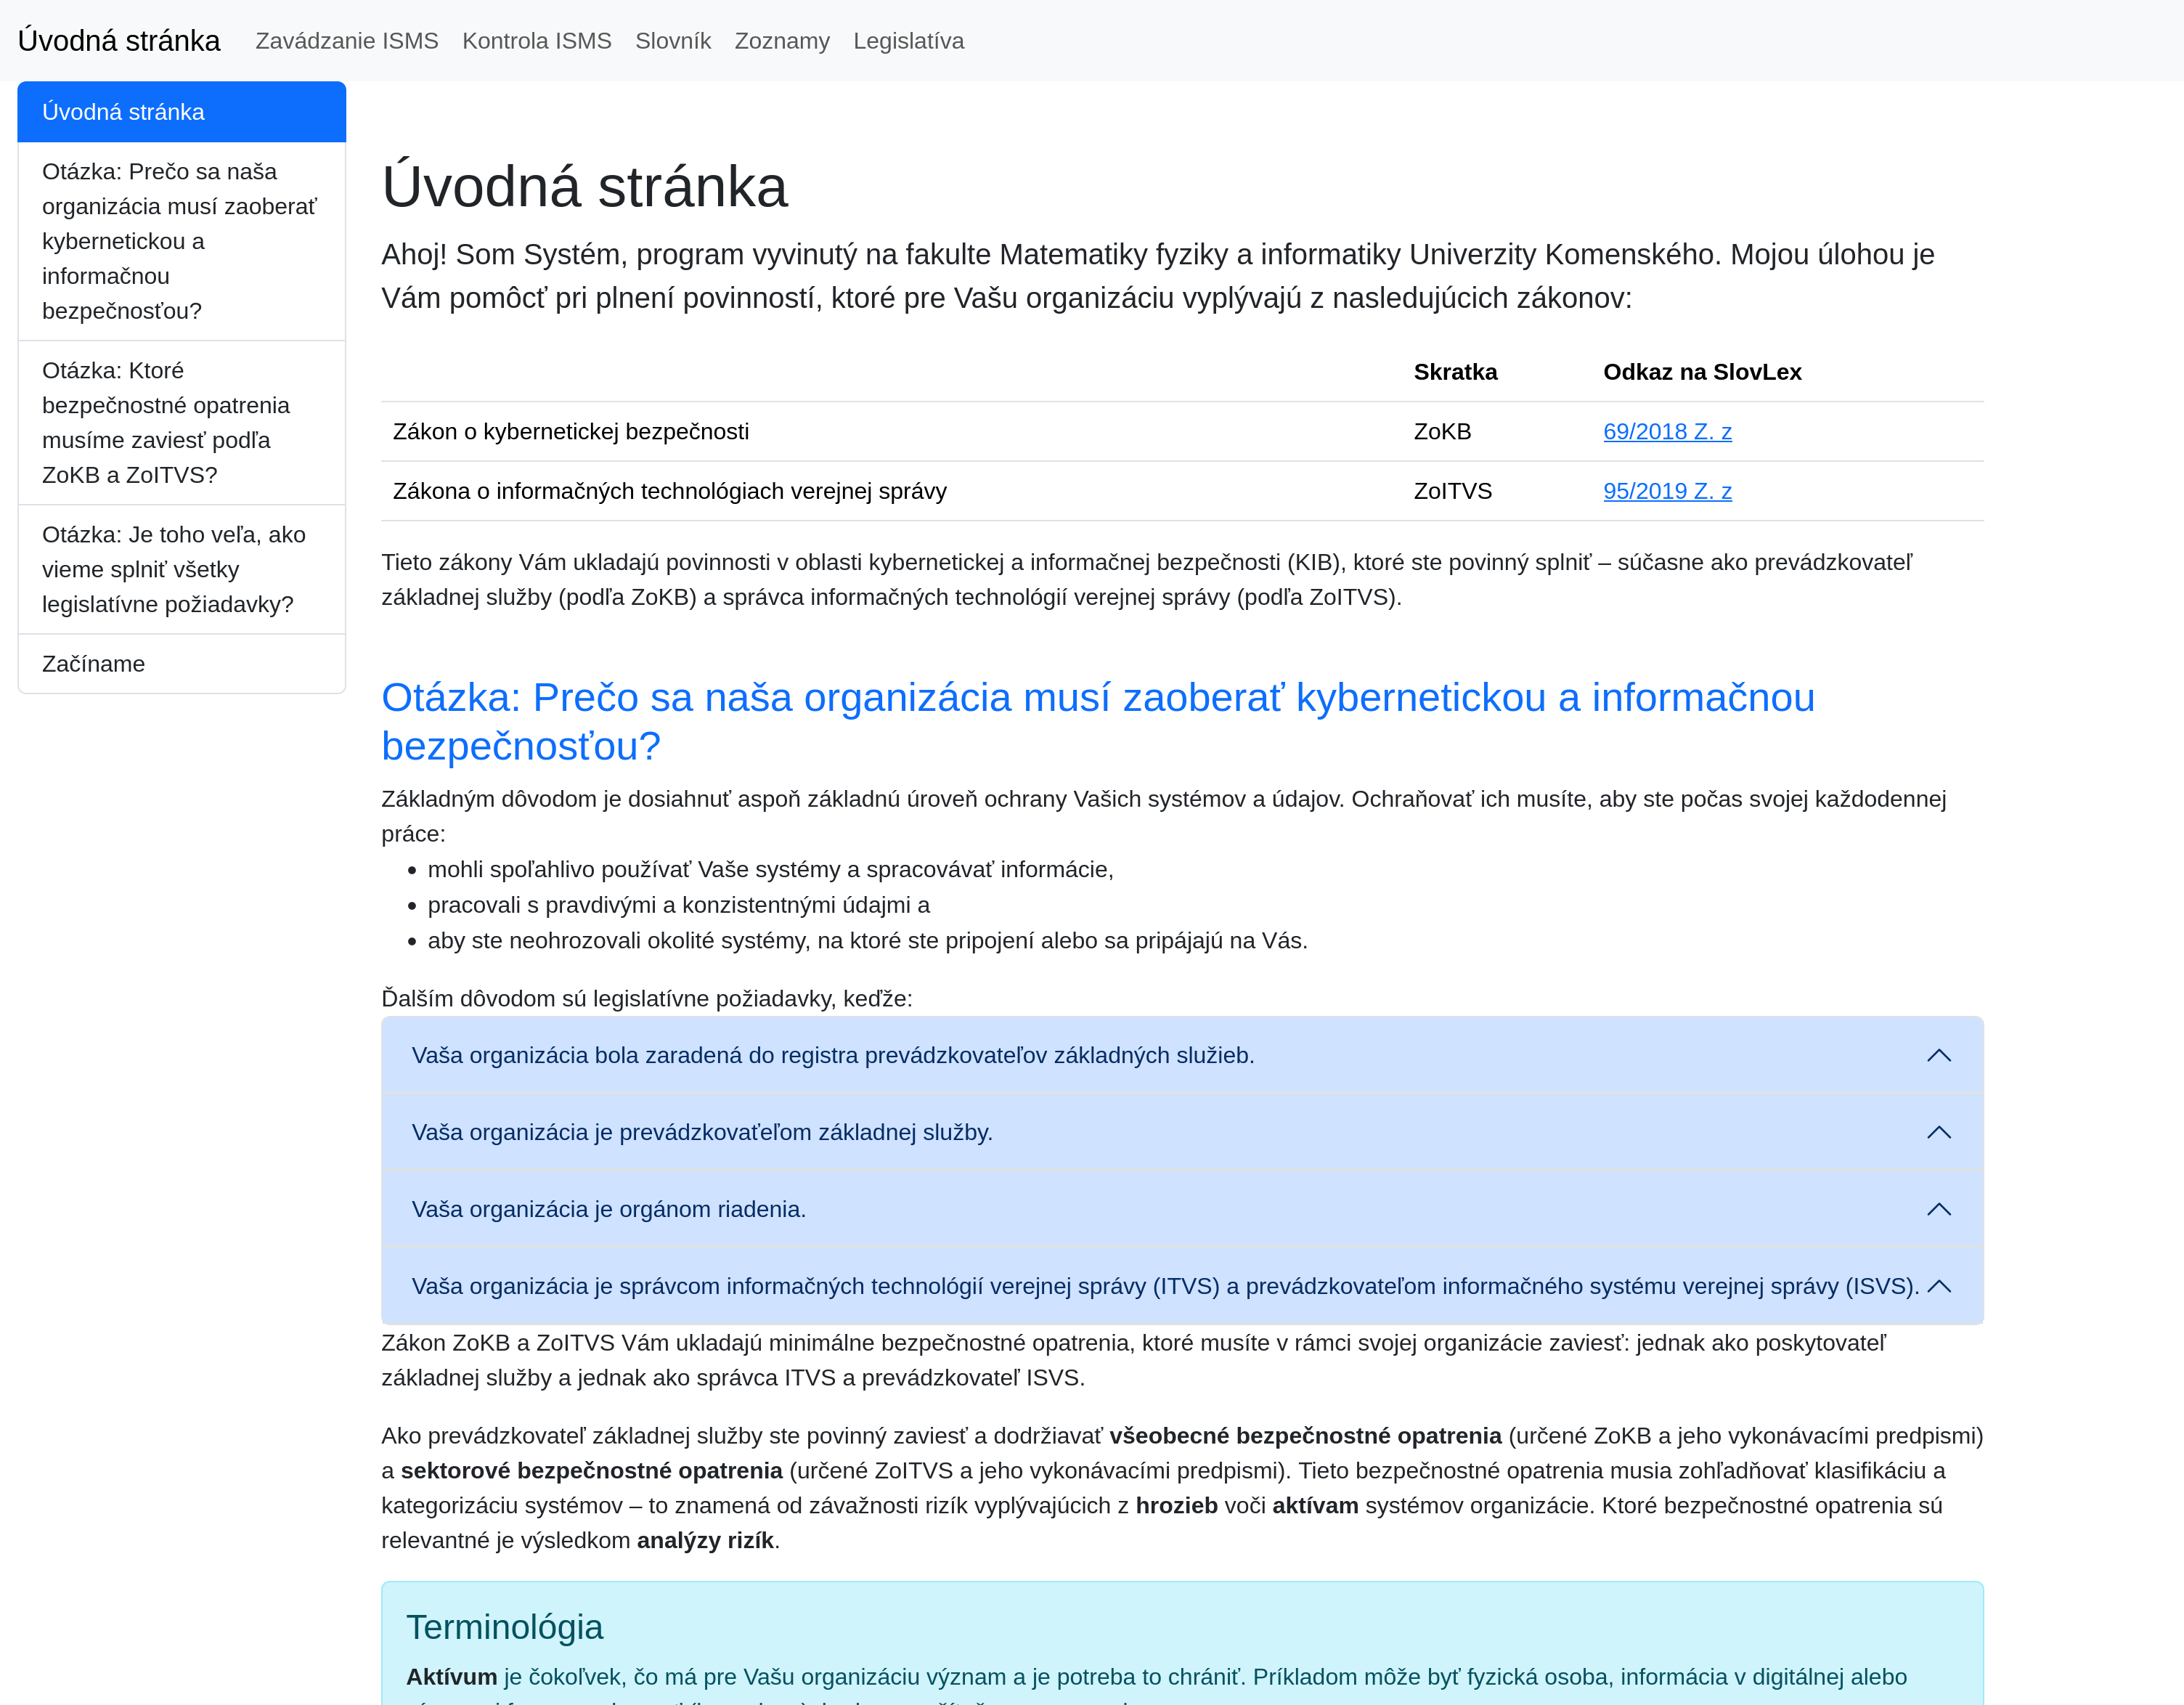
\includegraphics[width=0.85 \textwidth]{images/isms-uvodna-stranka}
  \caption{Úvodná stránka}
  \label{fig:isms-uvodna-stranka}
\end{figure}

\begin{figure}[h]
  \centering
  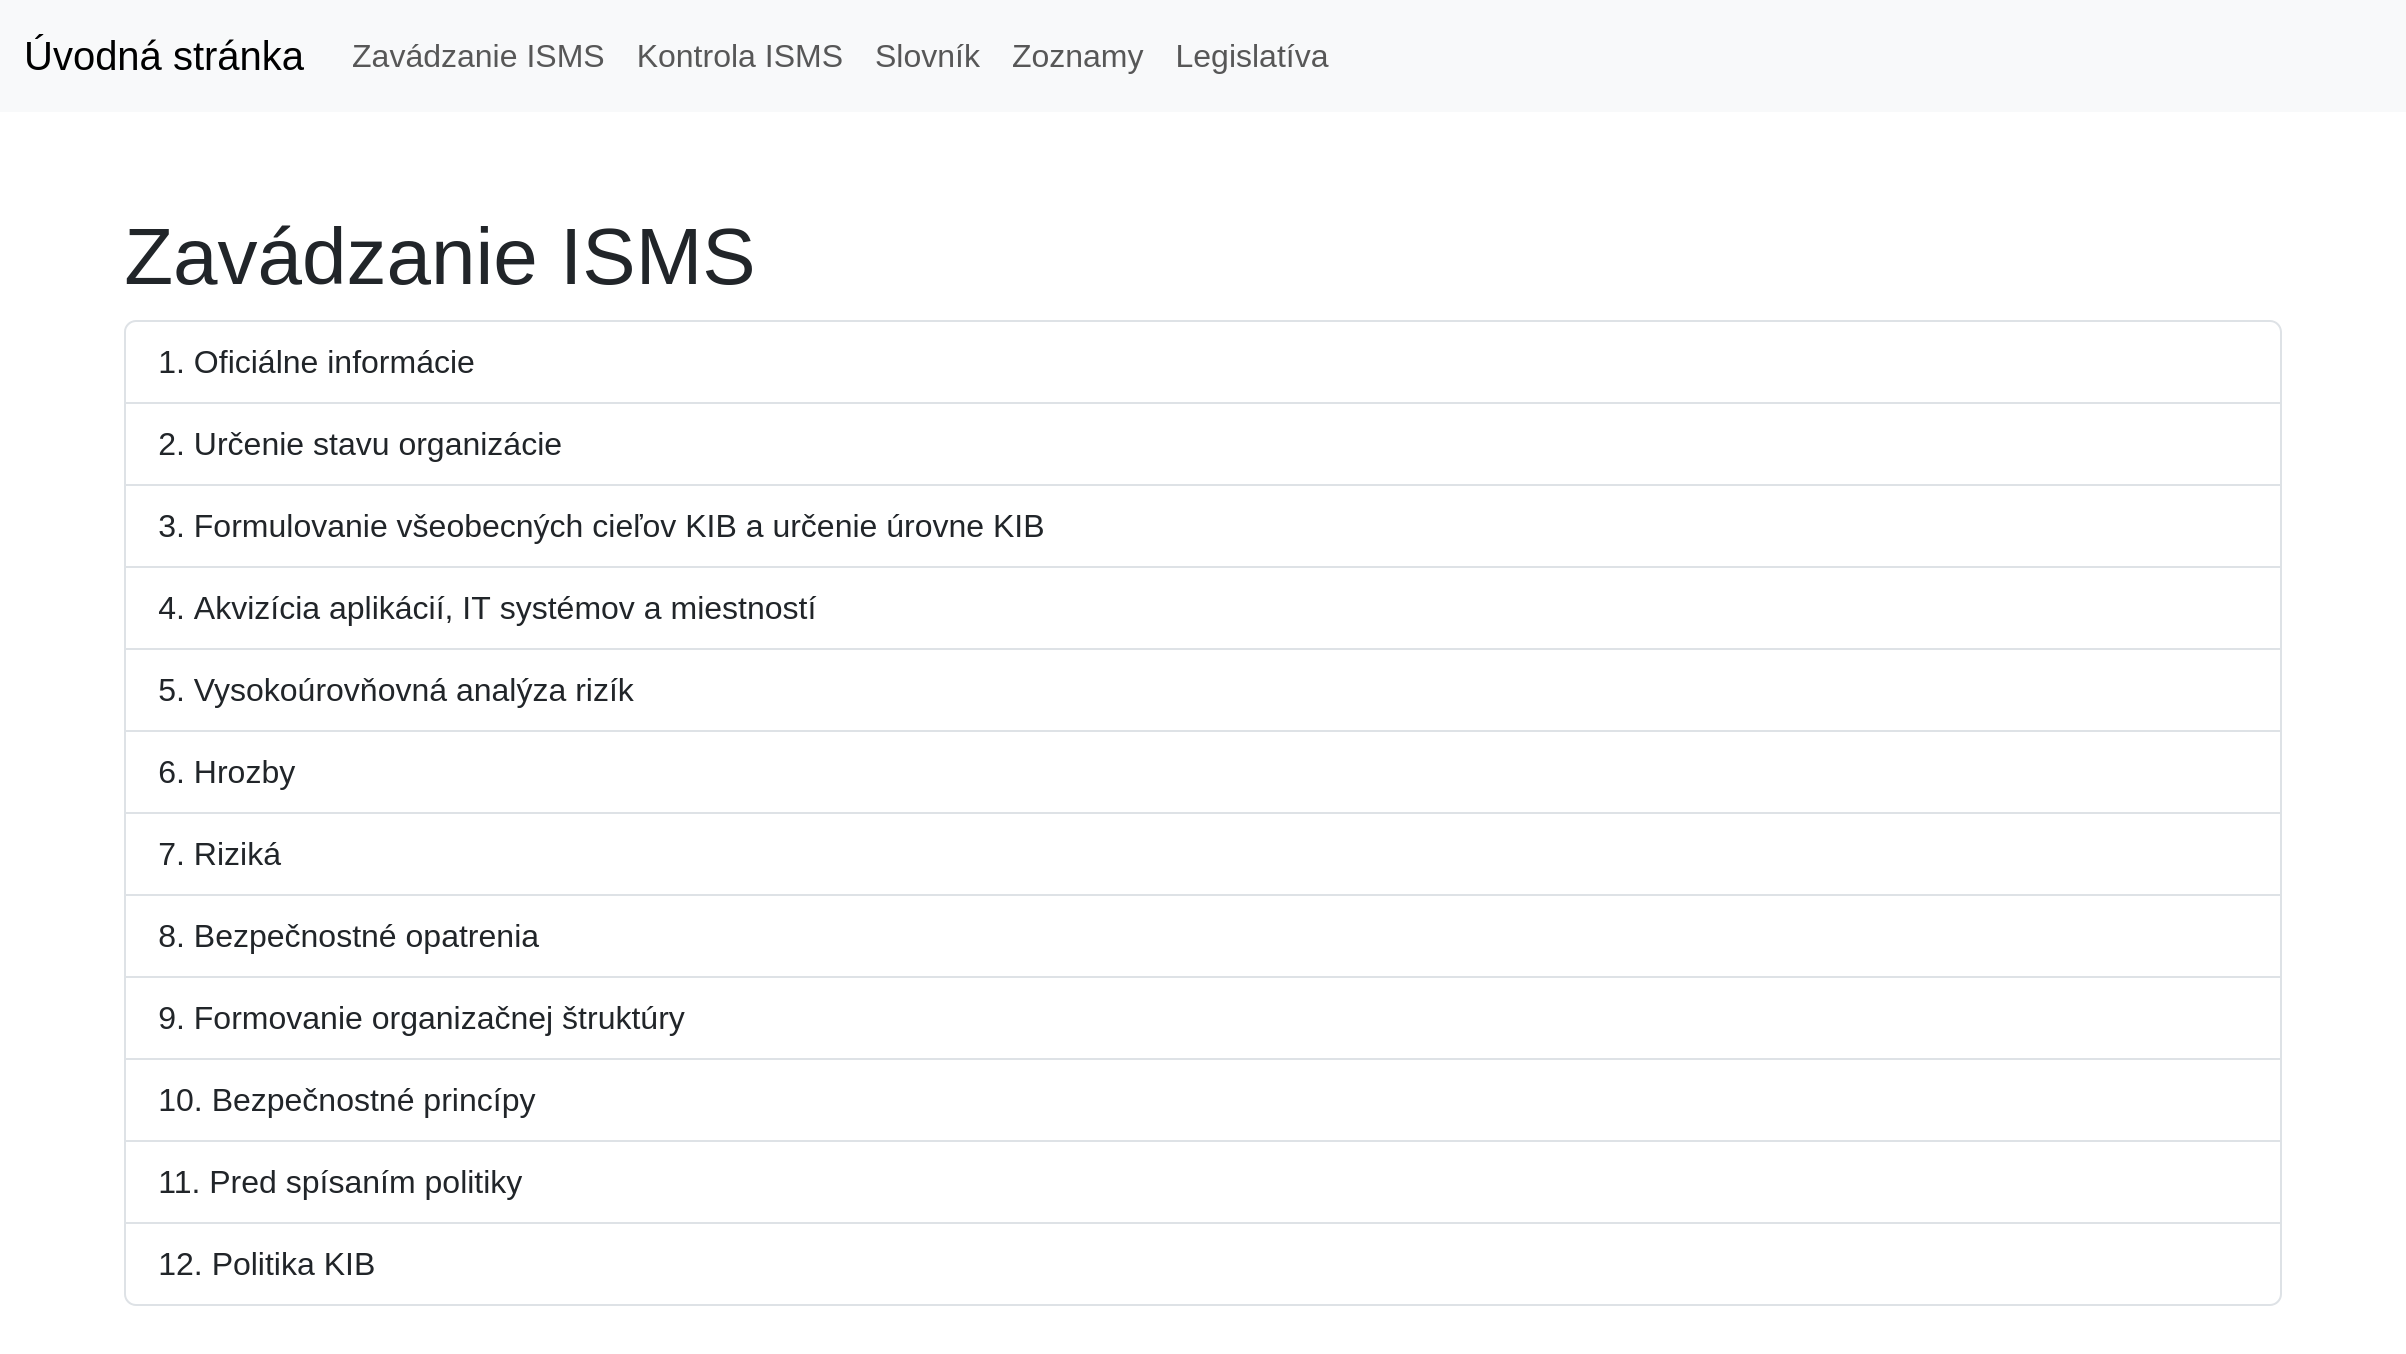
\includegraphics[width=0.85 \textwidth]{images/isms-setup-stranka}
  \caption{Stránka s návodom}
  \label{fig:isms-setup}
\end{figure}

Ďalej si prejdeme obsah každej časti s krátkym komentárom.

\subsection*{Systém: Úvodná stránka}
Na úvodnej stránke (obr. \ref{fig:isms-uvodna-stranka}) predstavíme náš systém, uvedieme používateľa do problematiky a
predstavíme mu zákony, ktoré sa ho týkajú -- ZoKB a ZoITVS. Pokračujeme metódou otázok, kde odhadneme, čo by sa manažér
KIB mohol opýtať. Najprv manažérovi KIB vysvetlíme, prečo sa v organizácii musia zaoberať KIB (morálne a legislatívne
dôvody) a vhodne to odôvodníme.

Po tom, ako vysvetlíme potrebu venovať sa KIB, by prišla prirodzená otázka -- Čo všetko musia (v očiach zákona) urobiť,
aby v dostatočnej miere splnili zákonné požiadavky? Zľahka manažérovi KIB predložíme požiadavky ZoKB a ZoITVS, pričom ich 
odkážeme na relevantné paragrafy (odkazujeme na portál Slov-lex).
\subsection*{Systém: } 
\subsection*{Systém: } 
\subsection*{Systém: } 
